%% Преамбула TeX-файла

% 1. Стиль и язык
\documentclass[utf8x, 14pt]{G7-32} % Стиль (по умолчанию будет 14pt)

% Остальные стандартные настройки убраны в preamble.inc.tex.
\sloppy

% Настройки стиля ГОСТ 7-32
% Для начала определяем, хотим мы или нет, чтобы рисунки и таблицы нумеровались в пределах раздела, или нам нужна сквозная нумерация.
\EqInChapter % формулы будут нумероваться в пределах раздела
\TableInChapter % таблицы будут нумероваться в пределах раздела
\PicInChapter % рисунки будут нумероваться в пределах раздела

% Добавляем гипертекстовое оглавление в PDF
\usepackage[
bookmarks=true, colorlinks=true, unicode=true,
urlcolor=black,linkcolor=black, anchorcolor=black,
citecolor=black, menucolor=black, filecolor=black,
]{hyperref}
\usepackage{pgfplots}
\usepackage{nomencl}

\usepackage{float}

\AfterHyperrefFix

\usepackage{microtype}% полезный пакет для микротипографии, увы под xelatex мало чего умеет, но под pdflatex хорошо улучшает читаемость
\usepackage{indentfirst}

% Тире могут быть невидимы в Adobe Reader
\ifInvisibleDashes
\MakeDashesBold
\fi

\usepackage{graphicx}   % Пакет для включения рисунков

% С такими оно полями оно работает по-умолчанию:
% \RequirePackage[left=20mm,right=10mm,top=20mm,bottom=20mm,headsep=0pt,includefoot]{geometry}
% Если вас тошнит от поля в 10мм --- увеличивайте до 20-ти, ну и про переплёт не забывайте:
\geometry{right=10mm}
\geometry{left=30mm}
\geometry{bottom=20mm}
\geometry{ignorefoot}% считать от нижней границы текста


% Пакет Tikz
\usepackage{tikz}
\usetikzlibrary{arrows,positioning,shadows}

% Произвольная нумерация списков.
\usepackage{enumerate}

% ячейки в несколько строчек
\usepackage{multirow}

% itemize внутри tabular
\usepackage{paralist,array}

%\setlength{\parskip}{1ex plus0.5ex minus0.5ex} % разрыв между абзацами
\setlength{\parskip}{1ex} % разрыв между абзацами
\usepackage{blindtext}

% Центрирование подписей к плавающим окружениям
%\usepackage[justification=centering]{caption}

\usepackage{newfloat}
\DeclareFloatingEnvironment[
placement={!ht},
name=Equation
]{eqndescNoIndent}
\edef\fixEqndesc{\noexpand\setlength{\noexpand\parindent}{\the\parindent}\noexpand\setlength{\noexpand\parskip}{\the\parskip}}
\newenvironment{eqndesc}[1][!ht]{%
    \begin{eqndescNoIndent}[#1]%
\fixEqndesc%
}
{\end{eqndescNoIndent}}

\usepackage{afterpage}

\newcommand\blankpage{
	\null
	\thispagestyle{empty}
	\newpage
}



% Настройки листингов.
\ifPDFTeX
% 8 Листинги

\usepackage{listings}

% Значения по умолчанию
\lstset{
  basicstyle= \footnotesize,
  breakatwhitespace=true,% разрыв строк только на whitespacce
  breaklines=true,       % переносить длинные строки
%   captionpos=b,          % подписи снизу -- вроде не надо
  inputencoding=koi8-r,
  numbers=left,          % нумерация слева
  numberstyle=\footnotesize,
  showspaces=false,      % показывать пробелы подчеркиваниями -- идиотизм 70-х годов
  showstringspaces=false,
  showtabs=false,        % и табы тоже
  stepnumber=1,
  tabsize=4,              % кому нужны табы по 8 символов?
  frame=single,
  xleftmargin=2.4em,
  framexleftmargin=2em
}

% Стиль для псевдокода: строчки обычно короткие, поэтому размер шрифта побольше
\lstdefinestyle{pseudocode}{
  basicstyle=\small,
  keywordstyle=\color{black}\bfseries\underbar,
  language=Pseudocode,
  numberstyle=\footnotesize,
  commentstyle=\footnotesize\it
}

% Стиль для обычного кода: маленький шрифт
\lstdefinestyle{realcode}{
  basicstyle=\scriptsize,
  numberstyle=\footnotesize
}

% Стиль для коротких кусков обычного кода: средний шрифт
\lstdefinestyle{simplecode}{
  basicstyle=\footnotesize,
  numberstyle=\footnotesize
}

% Стиль для BNF
\lstdefinestyle{grammar}{
  basicstyle=\footnotesize,
  numberstyle=\footnotesize,
  stringstyle=\bfseries\ttfamily,
  language=BNF
}

% Определим свой язык для написания псевдокодов на основе Python
\lstdefinelanguage[]{Pseudocode}[]{Python}{
  morekeywords={each,empty,wait,do},% ключевые слова добавлять сюда
  morecomment=[s]{\{}{\}},% комменты {а-ля Pascal} смотрятся нагляднее
  literate=% а сюда добавлять операторы, которые хотите отображать как мат. символы
    {->}{\ensuremath{$\rightarrow$}~}2%
    {<-}{\ensuremath{$\leftarrow$}~}2%
    {:=}{\ensuremath{$\leftarrow$}~}2%
    {<--}{\ensuremath{$\Longleftarrow$}~}2%
}[keywords,comments]

% Свой язык для задания грамматик в BNF
\lstdefinelanguage[]{BNF}[]{}{
  morekeywords={},
  morecomment=[s]{@}{@},
  morestring=[b]",%
  literate=%
    {->}{\ensuremath{$\rightarrow$}~}2%
    {*}{\ensuremath{$^*$}~}2%
    {+}{\ensuremath{$^+$}~}2%
    {|}{\ensuremath{$|$}~}2%
}[keywords,comments,strings]

% Подписи к листингам на русском языке.
\renewcommand\lstlistingname{Листинг}
\renewcommand\lstlistlistingname{Листинги}

\else
\usepackage{local-minted}
\fi

% Полезные макросы листингов.
% Любимые команды
\newcommand{\Code}[1]{\textbf{#1}}


% Стиль титульного листа и заголовки

%\NirEkz{Экз. 3}                                  % Раскоментировать если не требуется
%\NirGrif{Секретно}                % Наименование грифа

%\gosttitle{Gost7-32}       % Шаблон титульной страницы, по умолчанию будет ГОСТ 7.32-2001, 
% Варианты GostRV15-110 или Gost7-32 
 
\NirOrgLongName{ 
МОСКОВСКИЙ ГОСУДАРСТВЕННЫЙ ТЕХНИЧЕСКИЙ УНИВЕРСИТЕТ ИМ. Н. Э. БАУМАНА
}                                           %% Полное название организации

\NirUdk{УДК № 004.822}
%\NirGosNo{№ госрегистрации }
%\NirInventarNo{Инв. № ??????}

%\NirConfirm{Согласовано}                  % Смена УТВЕРЖДАЮ
\NirBoss[.49]{Проректор университета\\по научной работе}{В.Н. Зимин.}            %% Заказчик, утверждающий НИР


%\NirReportName{Научно-технический отчет}   % Можно поменять тип отчета
%\NirAbout{О составной части \par опытно-конструкторской работы} %Можно изменить о чем отчет

%\NirPartNum{Часть}{1}                      % Часть номер

%\NirBareSubject{}                  % Убирает по теме если раскоментить

% \NirIsAnnotacion{АННОТАЦИОННЫЙ }         %% Раскомментируйте, если это аннотационный отчёт
%\NirStage{промежуточный}{Этап \No 1}{} %%% Этап НИР: {номер этапа}{вид отчёта - промежуточный или заключительный}{название этапа}
%\NirStage{}{}{} %%% Этап НИР: {номер этапа}{вид отчёта - промежуточный или 

\Nir{}

\NirSubject{Драйвер нулевого уровня для использования графического планшета в качестве клавиатуры}                % Наименование темы
%\NirFinal{}                        % Заключительный, если закоментировать то промежуточный
%\finalname{итоговый}               % Название финального отчета (Заключительный)
%\NirCode{Шифр\,---\,САПР-РЛС-ФИЗТЕХ-1} % Можно задать шифр как в ГОСТ 15.110
\NirCode{}

% \NirManager{Зам. проректора по научной работе}{Р.А. Бадамшин  } %% Название руководителя
\NirIsp{Руководитель темы}{Кирилл Леонидович Тассов} %% Название руководителя

\NirYear{2020}%% если нужно поменять год отчёта; если закомментировано, ставится текущий год
\NirTown{Москва}                           %% город, в котором написан отчёт


\usepackage{pdfpages}

\begin{document}

\frontmatter % выключает нумерацию ВСЕГО; здесь начинаются ненумерованные главы: реферат, введение, глоссарий, сокращения и прочее.

%\maketitle %создает титульную страницу

\includepdf[pages=-]{pages/title.pdf}
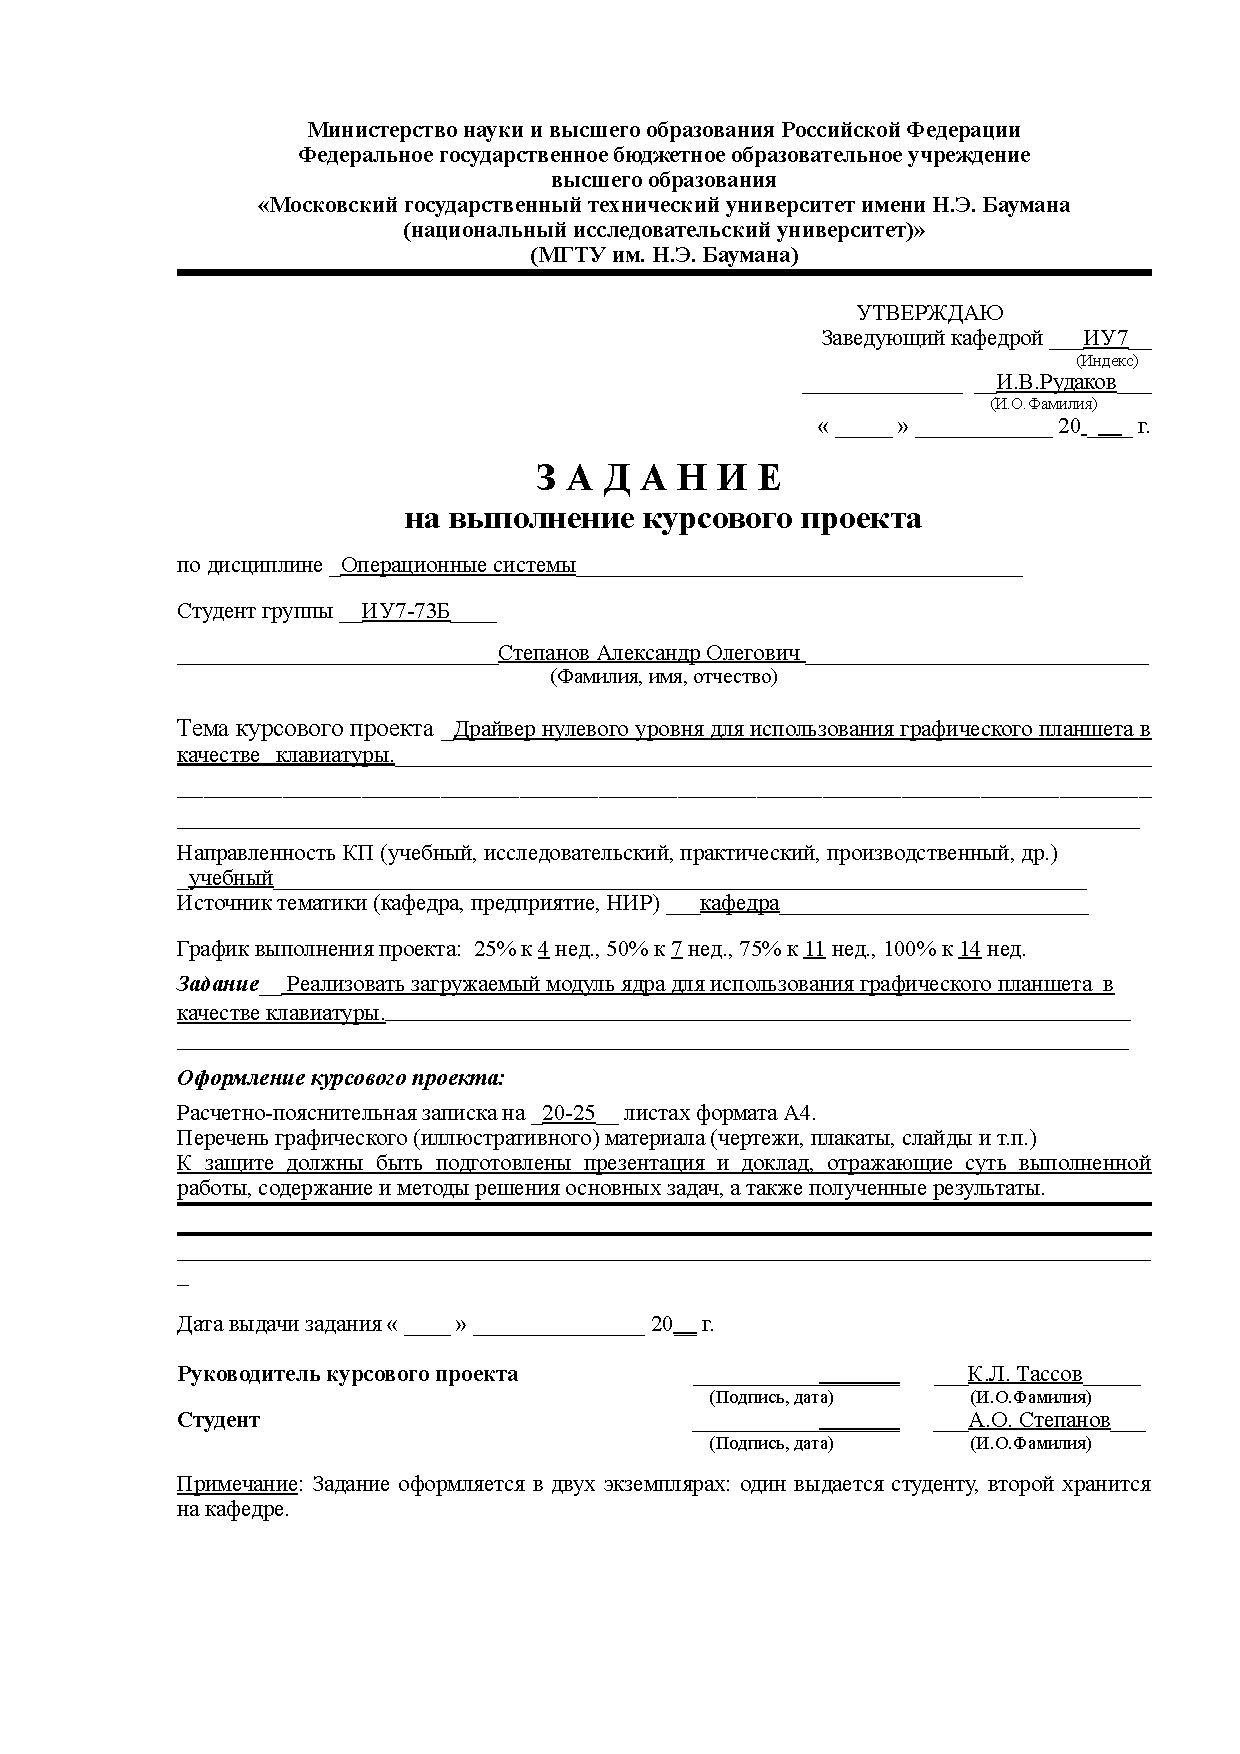
\includepdf[pages=-]{pages/tz.pdf}
% пропущены страницы под тз и план (у меня их 2 тз и 1 план, итого 3, вам надо пропустить столько, сколько страниц у вас в тз и плане)


%\listoffigures                         % Список рисунков

%\listoftables                          % Список таблиц

%\NormRefs % Нормативные ссылки 
% Команды \breakingbeforechapters и \nonbreakingbeforechapters
% управляют разрывом страницы перед главами.
% По-умолчанию страница разрывается.

\Referat
%\begin{abstract}

    Отчет содержит \pageref{LastPage}\,стр.%
    \ifnum \totfig >0
    , \totfig~рис.%
    \fi
    \ifnum \tottab >0
    , \tottab~табл.%
    \fi
    %
    \ifnum \totbib >0
    , \totbib~источн.%
    \fi
    %
    \ifnum \totapp >0
    , \totapp~прил.%
    \else
    .%
    \fi

    Ключевые слова: linux, драйвер, графический планшет, загружаемый модуль ядра, клавиатура, прерывания, пространство ядра.

    Курсовой проект представляет собой загружаемый модуль ядра для использования графического планшета в качестве клавиатуры. Используется язык программирования C.

%\end{abstract}

%%% Local Variables:
%%% mode: latex
%%% TeX-master: "rpz"
%%% End:

% \nobreakingbeforechapters
% \breakingbeforechapters

\tableofcontents

% \printnomenclature % Автоматический список сокращений

\Introduction



\mainmatter % это включает нумерацию глав и секций в документе ниже

\chapter{Аналитический раздел}
\label{cha:analysis}


\chapter{Конструкторский раздел}
\label{cha:design}

В данном разделе рассматривается структура программного обеспечения.

\section{Состав программного обеспечения}

Программное обеспечение состоит из загружаемого модуля ядра.

\subsection{Загрузка модуля ядра}

Для компиляции модуля используется специальный makefile. На листинге \ref{lst:make} представлен makefile, с помощью которого компилировался модуль ядра из данной работы.

\begin{lstlisting}[language=make,caption=Makefile для компиляции модуля ядра,label=lst:make]
ifneq ($(KERNELRELEASE),)
    obj-m := keyboard_tablet.o
else
    CURRENT = $(shell uname -r)
    KDIR = /lib/modules/$(CURRENT)/build
    PWD = $(shell pwd)

all:
    $(MAKE) -C $(KDIR) M=$(PWD) modules

clean:
    @rm -f *.o .*.cmd .*.flags *.mod.c *.order
    @rm -f .*.*.cmd *~ *.*~ TODO.*
    @rm -fR .tmp*
    @rm -rf .tmp_versions

disclean: clean
    @rm *.ko *.symvers

endif
\end{lstlisting}

После компиляции получается объектный файл с расширением .ko, который можно загрузить в ядро с помощью команды insmod под sudo.

\section{Создание usb драйвера}

Для создания usb драйвера создается экземпляр структуры usb\_driver \cite{Usb_driver}. Создание экземпляра приведено на листинге \ref{lst:usb_driver}.

\begin{lstlisting}[language=c,caption=Создание экземпляра usb драйвера,label=lst:usb_driver]
static struct usb_driver tablet_driver = {
    .name       = DRIVER_NAME,
    .probe      = tablet_probe,
    .disconnect = tablet_disconnect,
    .id_table   = tablet_table,
};
\end{lstlisting}

Для ругистрации usb драйвера используется системный вызов usb\_register \cite{Usb_register}.

\section{Структура для хранения ифнормации о графическом планшете}

Для передачи данных, связанных с графическим планшетом была создана структура tablet, приведенная на листинге \ref{lst:tablet_t}.

\begin{lstlisting}[language=c,caption=Структура планшета,label=lst:tablet_t]
struct tablet {
    unsigned char     *data;
    struct input_dev  *input_dev;
    struct usb_device *usb_dev;
    struct urb        *irq;
};
typedef struct tablet tablet_t;
\end{lstlisting}

В данной структуре созданы следующие поля:

\begin{itemize}
    \item data -- данные, передаваемые планшетом при прерывании;
    \item input\_dev -- подключенный планшет;
    \item usb\_dev -- представление usb устройства;
    \item irq -- обработчик прерываний.
\end{itemize}

\section{Структура для передачи данных о прерывании}

Для того, чтобы передавать в работу из очереди данные о прерывании была создана структура container\_urb, представленная на листинге \ref{lst:container_urb}.

\begin{lstlisting}[language=c,caption=Структура для передачи данных о прерывании,label=lst:container_urb]
struct container_urb {
    struct urb *urb;
    struct work_struct work;
};

typedef struct container_urb container_urb_t;
\end{lstlisting}

В данной структуре созданы следующие поля:

\begin{itemize}
    \item urb -- обработанное прерывание;
    \item work -- текущая работа в очереди.
\end{itemize}

\section{Обработка прерываний}

На рисунке \ref{fig:urb} предствалена схема обработки прерываний графического планшета и отправка событий нажатия на клавиши клавиатуры.

\begin{figure}[H]
    \centering
    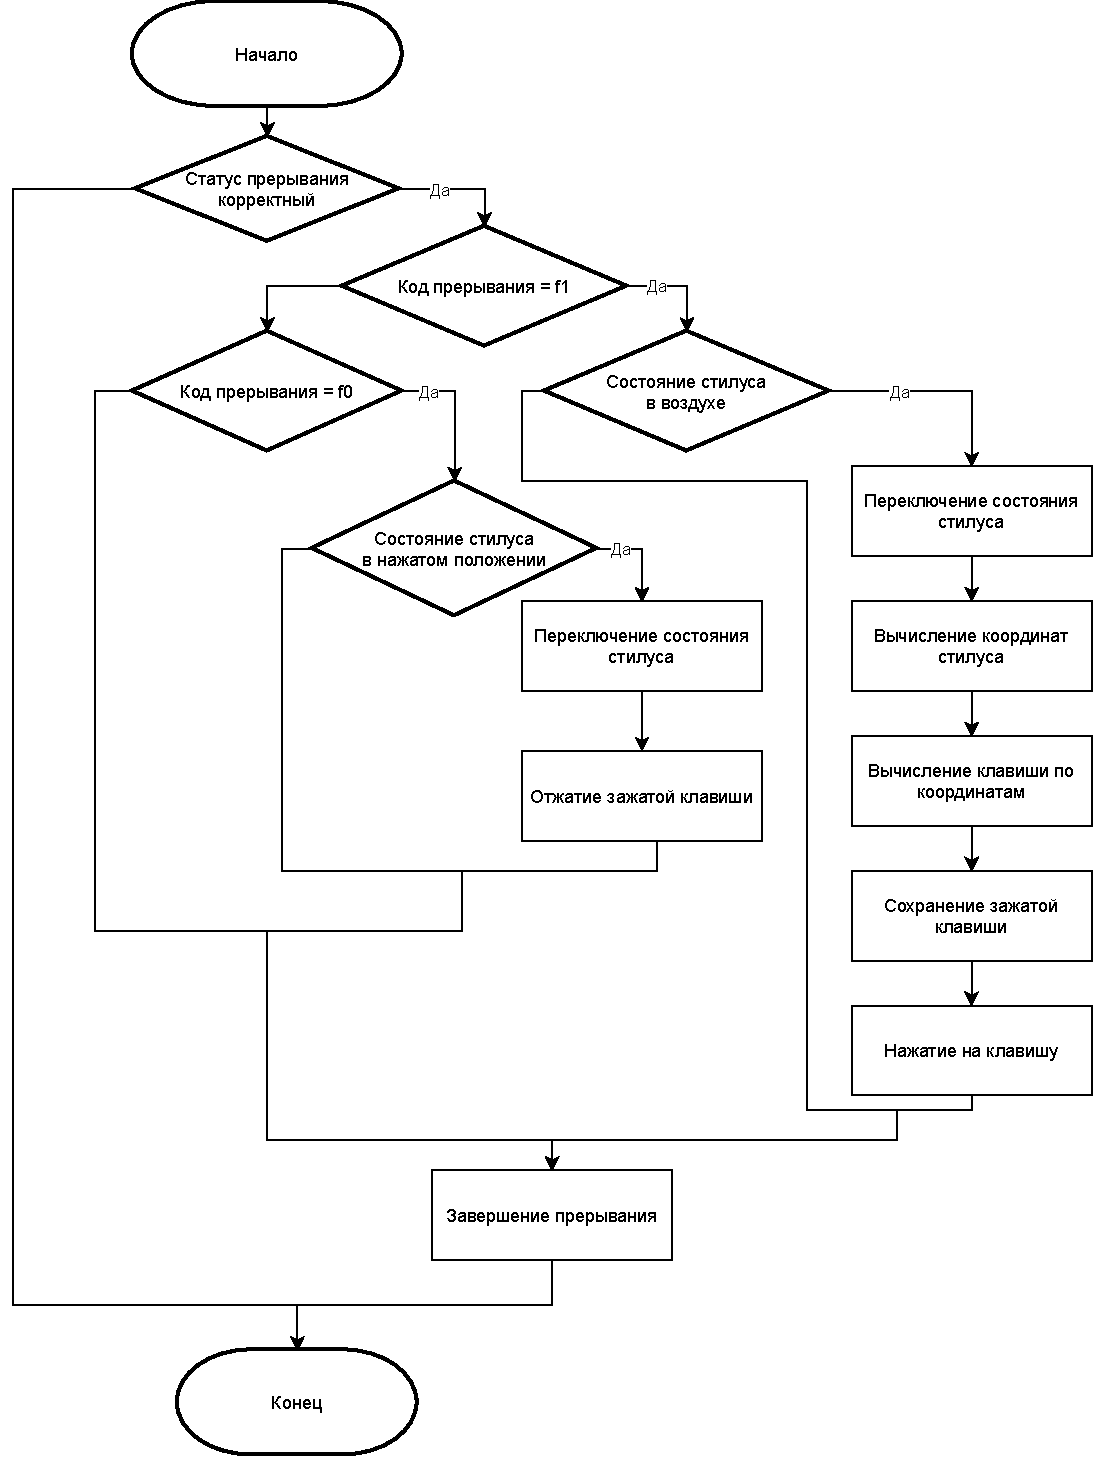
\includegraphics[width=0.9\textwidth]{img/urb.pdf}
    \caption{Обработка прерываний}
    \label{fig:urb}
\end{figure}

\section{Разделение поверхности планшета на клавиши}

Для комфортного использования модуля клавиши были расставлены на основе классической qwerty раскладки \cite{Qwerty}.

Координаты стилуса находятся в диапазоне от 0 до 1344 по оси x и от 0 до 468 по y. Поскольку координаты стилуса принимают только значения кратные 16 для оси x и кратные 9 для y, то поверхость была поделена на области размером 16 на 9. Таких областей получилось 84 на 52. Именно координаты этих областей и используются для вычисления клавиши. На рисунке \ref{fig:keyboard} представлена схема разделения поверхности планшета на клавиши клавиатуры.

\begin{figure}[H]
    \centering
    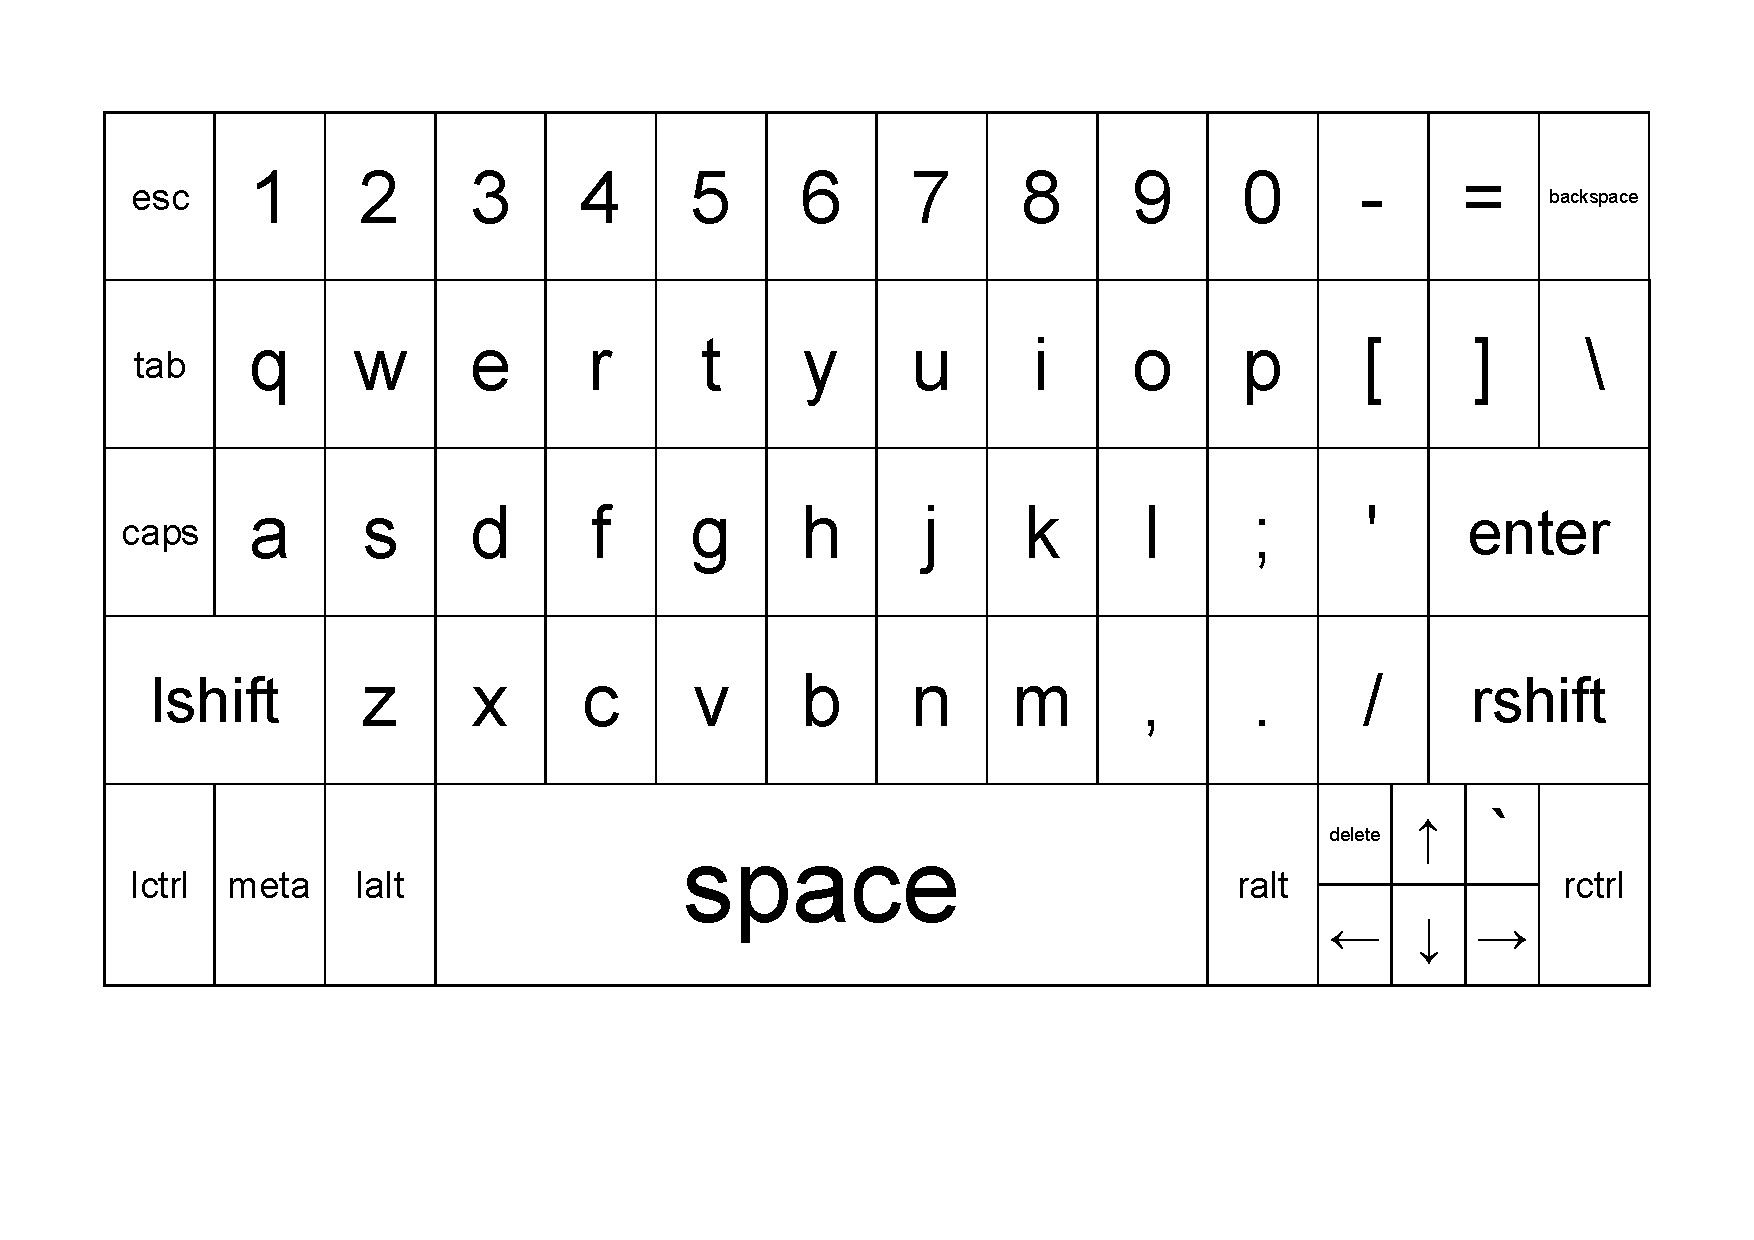
\includegraphics[trim=3cm 4cm 3cm 1.5cm, width=0.9\textwidth]{img/keyboard.pdf}
    \caption{Разделение поверхности планшета на клавиши}
    \label{fig:keyboard}
\end{figure}

\section{Вывод}

В данном разделе был рассмотрен процесс проектирования структуры программного обеспечения.

\chapter{Технологический раздел}
\label{cha:impl}

В данном разделе производится выбор средств для разработки и рассматривается реализация программного обеспечения.

\section{Выбор языка программирования}

В качестве языка программирования был выбран язык C. На этом языке реализованы все модули ядра и драйверы операционной системы Linux. Компилятор -- gcc.

\section{Работа программы}

Рассмотрим работу модуля с листингами.

\subsection{Начальная настройка}

На листинге \ref{lst:macros} представлено объявление всех необходимых макросов. На листинге \ref{lst:structs} представлено объявление всех глобальных пременных, а именно:

\begin{itemize}
    \item pen\_enter -- положение стилуса (на планшете или в воздухе);
    \item pressed\_key -- нажатая в текущий момент клавиша;
    \item workq -- очередь работ;
    \item keyboard -- виртуальное устрйоство для вывода событий клавиш.
\end{itemize}

Также там объявляются структуры tablet, которая нужна для хранения данных о состоянии планшета, и container\_urb, которая нужна для передачи данных о текущем прерывании в работу.

На листинге \ref{lst:init} представлена функция инициализации модуля, где происходит регистрация драйвера, инициализацяи очереди работ, настройка виртуального устройства клавиатуры и ее регистрация.

На листинге \ref{lst:exit} представлена функция выгрузки модуля, где происходит очистка памяти, выключение драйвера и удаление вртуального устройства.

\subsection{Драйвер для планшета}

На листинге \ref{lst:probe} представлена функция подключения планшета, в которой производится все необходимое выделение памяти и настрйока.

На листинге \ref{lst:input_dev_open_close} представлены функции открытия и закрытия устройства ввода.

На листинге \ref{lst:disconnect} представлена функция отключения планшета, в которой освобождается память и удаляются обработчики.

На листинге \ref{lst:device_id} представлена таблица устройств, которые необходимо подключать. Первый элемент этой таблицы это планшет Wacom Ltd CTL-671, который использовался для тестирования драйвера, а второй -- пустой элемент, это означает, что если нет устройства, у которого совпадают идентификаторы из других элементов таблицы, то драйвер будет пытаться подключить каждое свободное устройство.

На листинге \ref{lst:irq} представлена функция, которая перехватывает прерывание. В ней создается работа и отправляется в очередь обработки.

На листинге \ref{lst:work_irq} представлена функция, обрабатывающая прерывание. Ее алгоритм представлен на рисунке \ref{fig:urb}.

\subsection{Нажатие клавиш клавиатуры}

На листинге \ref{lst:keydown_keyup} представлены функции нажатия и отжатия текущей клавиши.

На листинге \ref{lst:press_key} представлена часть функции выбора клавиши в зависимости от координат. Разделение поверхности планшета на клавиши представлено на рисунке \ref{fig:keyboard}.

\section{Пример работы программы}

На рисунке \ref{fig:connect} изображены логи при подключении планшета в систему. В этот момент планшет также подключается и к драйверу.

\begin{figure}[H]
    \centering
    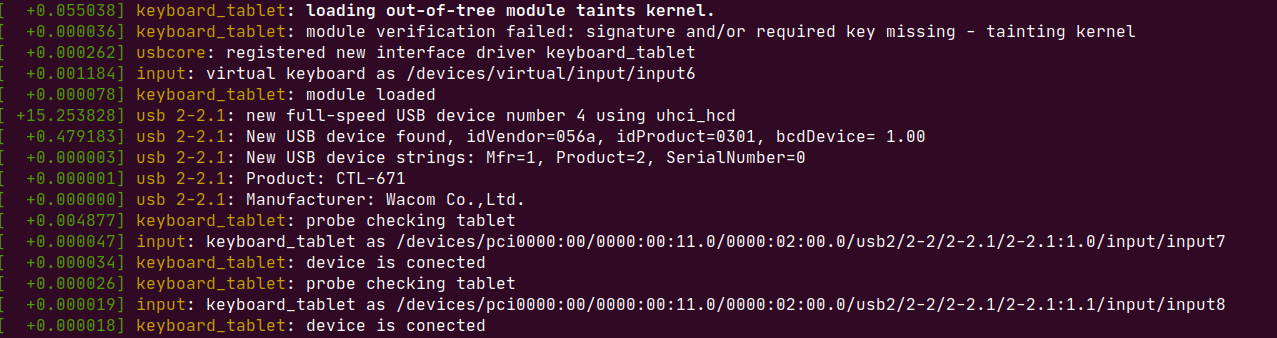
\includegraphics[width=0.8\textwidth]{img/connect.png}
    \caption{Подключение планшета к операционной системе}
    \label{fig:connect}
\end{figure}

На рисунке \ref{fig:work} изображены логи нажатий на планшет в разных областях.

\begin{figure}[H]
    \centering
    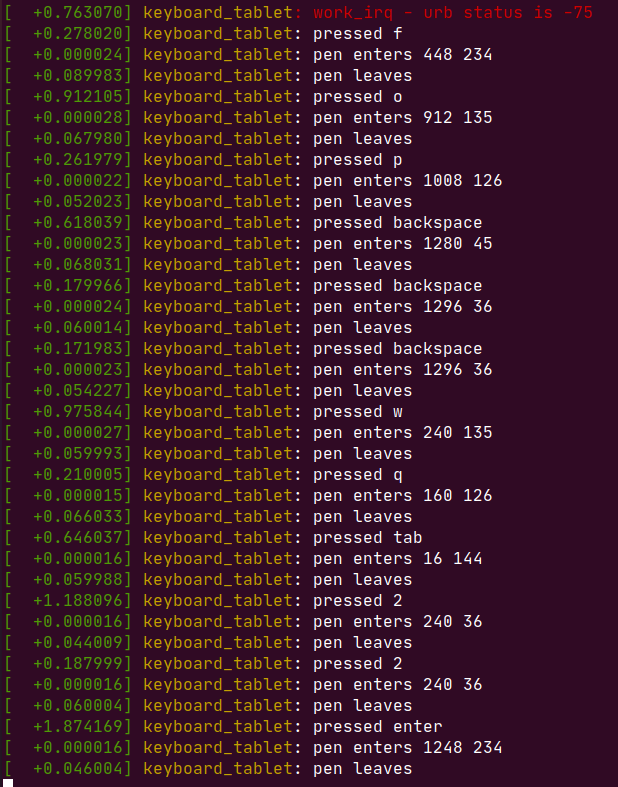
\includegraphics[width=0.8\textwidth]{img/work.png}
    \caption{Логи нажатий на планшет}
    \label{fig:work}
\end{figure}

На рисунке \ref{fig:work_wletters} изображены логи нажатий на планшет, когда открыта консоль с выводом логов. Здесь можно заметить перед сообщением о печати буквы сами эти буквы, которые были напечатаны с помощью планшета.

\begin{figure}[H]
    \centering
    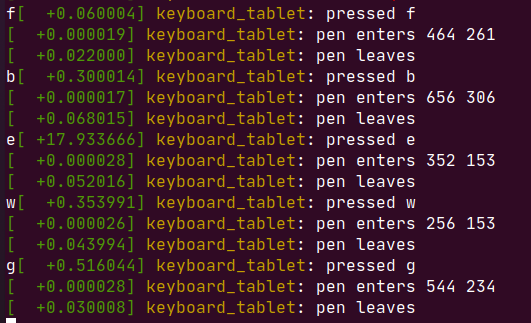
\includegraphics[width=0.8\textwidth]{img/work_wletters.png}
    \caption{Логи нажатий на планшет в консоли с логами}
    \label{fig:work_wletters}
\end{figure}

На рисунке \ref{fig:disconnect} изображены логи отключения планшета.

\begin{figure}[H]
    \centering
    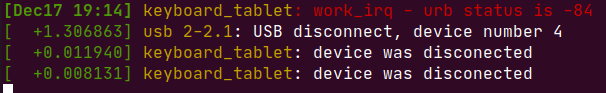
\includegraphics[width=0.8\textwidth]{img/disconnect.png}
    \caption{Отключение планшета от оперционной системы}
    \label{fig:disconnect}
\end{figure}

\section{Вывод}

В данном разделе был выбран язык программирования C, а также рассмотрена реализация программного обеспечения.

%\chapter{Исследовательский раздел}
\label{cha:research}



\backmatter %% Здесь заканчивается нумерованная часть документа и начинаются ссылки и
            
\Conclusion % заключение к отчёту

%% заключение


% % Список литературы при помощи BibTeX
% Юзать так:
%
% pdflatex rpz
% bibtex rpz
% pdflatex rpz

\bibliographystyle{ugost2008}
\bibliography{rpz}
\nocite{*}

%%% Local Variables: 
%%% mode: latex
%%% TeX-master: "rpz"
%%% End: 


%
\appendix   % Тут идут приложения
%
\chapter{Реализация и тестирование}

%
%\chapter{Еще картинки}
\label{cha:appendix2}
\blindtext

\begin{figure}
\centering
\caption{Еще одна картинка, ничем не лучше предыдущей. Но надо же как-то заполнить место.}
\end{figure}

%%% Local Variables: 
%%% mode: latex
%%% TeX-master: "rpz"
%%% End: 


\end{document}

%%% Local Variables:
%%% mode: latex
%%% TeX-master: t
%%% End:
